\documentclass[11pt]{aghdpl}
% \documentclass[en,11pt]{aghdpl}  % praca w języku angielskim

% Lista wszystkich języków stanowiących języki pozycji bibliograficznych użytych w pracy.
% (Zgodnie z zasadami tworzenia bibliografii każda pozycja powinna zostać utworzona zgodnie z zasadami języka, w którym dana publikacja została napisana.)
\usepackage[english,polish]{babel}

% Użyj polskiego łamania wyrazów (zamiast domyślnego angielskiego).
\usepackage{polski}

\usepackage[utf8]{inputenc}

% dodatkowe pakiety

\usepackage{mathtools}
\usepackage{float}
\usepackage{amsfonts}
\usepackage{amsmath}
\usepackage{textcomp}
\usepackage{amsthm}

% --- < bibliografia > ---

\usepackage[
style=numeric,
sorting=none,
%
% Zastosuj styl wpisu bibliograficznego właściwy językowi publikacji.
language=autobib,
autolang=other,
% Zapisuj datę dostępu do strony WWW w formacie RRRR-MM-DD.
urldate=iso8601,
% Nie dodawaj numerów stron, na których występuje cytowanie.
backref=false,
% Podawaj ISBN.
isbn=true,
% Nie podawaj URL-i, o ile nie jest to konieczne.
url=false,
%
% Ustawienia związane z polskimi normami dla bibliografii.
maxbibnames=3,
% Jeżeli używamy BibTeXa:
backend=bibtex
]{biblatex}

\usepackage{csquotes}
% Ponieważ `csquotes` nie posiada polskiego stylu, można skorzystać z mocno zbliżonego stylu chorwackiego.
\DeclareQuoteAlias{croatian}{polish}

\addbibresource{bibliografia.bib}

% Nie wyświetlaj wybranych pól.
%\AtEveryBibitem{\clearfield{note}}


% ------------------------
% --- < listingi > ---

% Użyj czcionki kroju Courier.
\usepackage{courier}

\usepackage{listings}
\lstloadlanguages{TeX}

\lstset{
	literate={ą}{{\k{a}}}1
           {ć}{{\'c}}1
           {ę}{{\k{e}}}1
           {ó}{{\'o}}1
           {ń}{{\'n}}1
           {ł}{{\l{}}}1
           {ś}{{\'s}}1
           {ź}{{\'z}}1
           {ż}{{\.z}}1
           {Ą}{{\k{A}}}1
           {Ć}{{\'C}}1
           {Ę}{{\k{E}}}1
           {Ó}{{\'O}}1
           {Ń}{{\'N}}1
           {Ł}{{\L{}}}1
           {Ś}{{\'S}}1
           {Ź}{{\'Z}}1
           {Ż}{{\.Z}}1,
	basicstyle=\footnotesize\ttfamily,
}

% ------------------------

\AtBeginDocument{
	\renewcommand{\tablename}{Tabela}
	\renewcommand{\figurename}{Rys.}
}

% ------------------------
% --- < tabele > ---

\usepackage{array}
\usepackage{tabularx}
\usepackage{multirow}
\usepackage{booktabs}
\usepackage{makecell}
\usepackage[flushleft]{threeparttable}

% defines the X column to use m (\parbox[c]) instead of p (`parbox[t]`)
\newcolumntype{C}[1]{>{\hsize=#1\hsize\centering\arraybackslash}X}


%---------------------------------------------------------------------------

\author{Szymon Nowak}
\shortauthor{Sz. Nowak}

%\titlePL{Przygotowanie bardzo długiej i pasjonującej pracy dyplomowej w~systemie~\LaTeX}
%\titleEN{Preparation of a very long and fascinating bachelor or master thesis in \LaTeX}

\titlePL{Sterowanie funkcjami inteligentnego budynku w oparciu o mapy przepływu użytkowników}
\titleEN{}


\shorttitlePL{Sterowanie funkcjami inteligentnego budynku w oparciu o mapy przepływu użytkowników} % skrócona wersja tytułu jeśli jest bardzo długi
\shorttitleEN{}

\thesistype{Praca dyplomowa inżynierska}
%\thesistype{Master of Science Thesis}

\supervisor{dr Dariusz Pałka}
%\supervisor{Marcin Szpyrka PhD, DSc}

\degreeprogramme{Informatyka}
%\degreeprogramme{Computer Science}

\date{2017}

\department{Katedra Informatyki Stosowanej}
%\department{Department of Applied Computer Science}

\faculty{Wydział Elektrotechniki, Automatyki,\protect\\[-1mm] Informatyki i Inżynierii Biomedycznej}
%\faculty{Faculty of Electrical Engineering, Automatics, Computer Science and Biomedical Engineering}

\acknowledgements{Brak podziękowań}


\setlength{\cftsecnumwidth}{10mm}

%---------------------------------------------------------------------------
\setcounter{secnumdepth}{4}
\brokenpenalty=10000\relax

\begin{document}

\titlepages

% Ponowne zdefiniowanie stylu `plain`, aby usunąć numer strony z pierwszej strony spisu treści i poszczególnych rozdziałów.
\fancypagestyle{plain}
{
	% Usuń nagłówek i stopkę
	\fancyhf{}
	% Usuń linie.
	\renewcommand{\headrulewidth}{0pt}
	\renewcommand{\footrulewidth}{0pt}
}

\setcounter{tocdepth}{2}
\tableofcontents
\clearpage

\chapter{Wprowadzenie}
\label{cha:wprowadzenie}

Brak wprowadzenia.

%---------------------------------------------------------------------------

\section{Cele pracy}
\label{sec:celePracy}

Brak celu.

%---------------------------------------------------------------------------

\section{Zawartość pracy}
\label{sec:zawartoscPracy}

Brak zawartości.



















\chapter{Określanie lokalizacji}
\label{cha:lokalizacja}
\section{Lokalizacja użytkownika}
Lokalizację użytkownika w systemie określa się na podstawie odległości od punktów, których współrzędne w przestrzeni trójwymiarowej są znane. Są to głównie routery i Beacony, jednak może się zdarzyć, że takim punktem staje się również inny użytkownik. Współrzędne użytkownika można obliczyć, dokonując pomiarów wskaźnika mocy \textit{RSSI}, podając siłę sygnałów odebranych przez otaczające go urządzenia i obliczając na ich podstawie dystans \cite{RSC}.
\section{Trilateracja}
Powszechnie wykorzystywanym sposobem obliczenia lokalizacji użytkownika na podstawie dystansu do znanych punktów, jest trilateracja \cite{MS}. Metoda ta polega na przedstawieniu dystansu dzielącego punkt od nadajników w postaci okręgi (lub sfery w przypadku, gdy określamy lokalizację w trzech wymiarach). Następnie, należy wyznaczyć współrzędne punktu przecięcia okręgów \cite{MS}. Wyznaczony punkt jest lokalizacją odbiornika, dla którego dokonywaliśmy obliczenia.
\begin{figure}[H]			
	\centering
	\caption{Wizualizacja modelu trilateracji}
	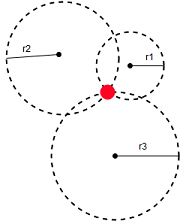
\includegraphics{trilateracja}
\end{figure}
Współrzędną punktu można obliczyć na podstawie wzoru:
\begin{equation}
\left\{
\begin{array}{l}
(x_p-x_1)^2 + (y_p - y_1)^2 = r_1^2\\
(x_p-x_2)^2 + (y_p - y_2)^2 = r_2^2\\
(x_p-x_3)^2 + (y_p - y_3)^2 = r_3^2
\end{array}
\right.
\end{equation}
gdzie:
\begin{itemize}
	\item $x_p$, $y_p$ to współrzędne obliczanego odbiornika
	\item $x_1$, $y_1$, $x_2$, $y_2$, $x_3$, $y_3$ to współrzędne znanych punktów
	\item $r_1$, $r_2$, $r_3$ to odległości między punktem obliczanym, a punktami o znanych współrzędnych
\end{itemize}
Ta metoda lokalizowania użytkownika w przestrzeni ma jedną, bardzo ważną wadę, która wyklucza jej wykorzystanie w tworzonym systemie - nie potrafi się dostosować do błędów pomiarowych, których w przypadku określania lokalizacji przy użyciu sygnałów radiowych, jest dużo. Aby wyznaczone lokalizacje użytkowników w sposób zbliżony odwzorowywały rzeczywiste położenie, algorytm obliczający musiał być bardziej odporny na błędy pomiarowe \cite{MT}.
\section{Lokalizacja jako funkcja probabilistyczna Gaussa}
Z racji tego, iż mierzony sygnał, odbierany przez odbiornik, ulega zniekształceniom i odbiciom, określenie dystansu między transmiterem, a odbiorcą w sposób liniowy jest niezgodne z fizycznymi zachowaniami sygnału. Siła sygnału oraz straty wywołane przez zniekształcenia i odbicia, określone są w jednostce dB. Wynika z tego, że najlepszym przybliżeniem zmian siły sygnału może być funkcja Gaussa \cite{GMBF}. Zamiast określać konkretne położenie użytkownika, w pracy zastosowane będzie podejście, które pozwoli na przedstawienie jego lokalizacji jako prawdopodobieństwo położenia.\\
\subsection{Funkcja probabilistyczna Gaussa}
Funkcja probabilistyczna Gaussa jest to krzywa w kształcie dzwonu, symetryczna względem średniej $\mu$ oraz uzyskująca wartość maksymalną w punkcie $\frac{1}{\sqrt{2\pi}\sigma}$.
Określa się ją za pomocą wzoru:
\begin{equation}
F(x) = \frac{1}{\sigma\sqrt{2\pi}}e^{\left(\frac{-(x-\mu)^2}{2\sigma^2}\right)}
\end{equation}
Zmienne $\mu$ będąca średnią, oraz $\sigma$ będąca odchyleniem standardowym, w pełni opisują tą funkcję \cite{MIR}.
\begin{figure}[H]			
	\centering
	\caption{Wykres funkcji Gaussa dla różnych wartości parametrów}
	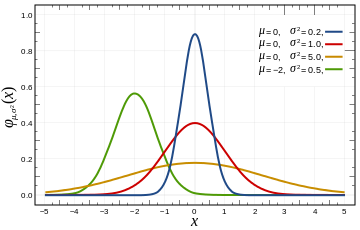
\includegraphics{funkcja_Gaussa}
\end{figure}
Funkcja Gaussa jest szeroko wykorzystywana w statystyce. W elektronice, korzysta się z niej podczas charakteryzowania pomiarów sensorów czy siły sygnałów radiowych.
\subsection{Model routerów jako funkcja Gaussa}
Jeżeli określimy lokalizację odbiornika względem transmitera jako funkcję prawdopodobieństwa Gaussa:
\begin{equation}
F(x) = \frac{1}{\sigma\sqrt{2\pi}}e^{\left(\frac{-(x-d)^2}{2\sigma^2}\right)}
\end{equation}
to wartość funkcji określa, jakie jest prawdopodobieństwo, że odbiornik znajduje się w odległości $x$ od transmitera. Największe prawdopodobieństwo przypisywane jest dystansowi, który obliczyliśmy z siły sygnału, dlatego to właśnie ta wartość podstawiana jest pod zmienną $d$. \cite{JK}\\
Jeżeli transmiter opisze się jako funkcję prawdopodobieństwa Gaussa \cite{YX}, wyznaczoną na podstawie odebranej siły sygnału, zwizualizowany model transmitera w przestrzeni dwuwymiarowej przypomina pierścień, którego gęstość maleje wraz z oddalaniem się od obliczonej z mocy sygnału odległości.
\begin{figure}[H]			
	\centering
	\caption{Wizualizacja modelu routera opisanego funkcją Gaussa. Jasność punktów oznacza wielkość prawdopodobieństwa $F(x)$. Na czerwono zaznaczono odległość obliczoną na podstawie siły sygnału transmitera $d$, a zielony prostokąt oznacza lokalizację transmitera.}
	
\includegraphics[width=0.75\textwidth]{router_Gaussa_wizualizacja}
\end{figure}
\subsection{Lokalizacja użytkownika opisana funkcją Gaussa}
Wyżej opisane podejście, poza realniejszym oddaniem natury rozchodzenia się sygnału w środowisku \cite{TDECHN}, ma również dodatkową zaletę - w łatwy sposób można wyliczyć prawdopodobieństwo położenia odbiornika wtedy, gdy w modelu znajduje się więcej transmiterów.\\
Jednym ze sposobów określenia położenia użytkownika jest zsumowanie prawdopodobieństw obliczonych w każdym punkcie w przestrzeni z funkcji Gaussa przypisanych do transmiterów. Prawdopodobieństwo dla puntu $(X,Y)$ może być określone na podstawie wzoru:
\begin{equation}
F(X,Y) = \sum_{r=1}^{R} \frac{1}{\sigma_r\sqrt{2\pi}}e^{\left(\frac{-(D(X,Y,r)-d_r)^2}{2\sigma_r^2}\right)}
\end{equation}
w którym kolejne symbol oznaczają:
\begin{itemize}
	\item $R$ - zbiór transmiterów. Z racji tego, iż funkcja Gaussa przyjmuje wartości większe od zera dla całego zakresu $(-\infty,\infty)$, wartość prawdopodobieństwa jest liczona dla każdego transmitera, niezależnie od tego, jak daleko znajduje się on od punktu $(X,Y)$
	\item $D(X,Y,r)$ - euklidesowa odległość punktu $(X,Y)$ od transmitera $r$
	\item $d_r$ - odległość obliczona na podstawie siły sygnału transmitera $r$
	\item $\sigma_r$ - odchylenie standardowe - wartość wyznaczana na podstawie odległości transmiterów od odbiornika. Dodatkowo, z racji tego, iż sygnał Wi-Fi jest bardziej odporny na nagłe zaniki wynikające ze wzrostu odległości, niż sygnał Bluetooth \cite{BLUE}, wartość odchylenia skalowana jest w zależności od tego, jaki typ sygnału wysyła konkretny transmiter.\\
	Wartość $sigma_r$ można obliczyć za pomocą wzoru:
	\begin{equation}
		sigma_r = \frac{D_m * w_r}{30}
	\end{equation}
	gdzie $D_m$ to długość najdłuższego boku modelu, tworzonego przez sygnały ze wszystkich transmiterów, a $w_r$ to waga sygnału, który wysyła transmiter $r$
\end{itemize}
Po ustaleniu wartości dla wszystkich punktów w przestrzeni, jako lokalizacja odbiornika przyjęty zostaje taki punkt $(X_o,Y_o)$, którego suma prawdopodobieństw jest najwyższa.
\begin{figure}[H]			
	\centering
	\caption{Model lokalizacji odbiornika wykonany w programie MatLab. Punkt o największym prawdopodobieństwie oznaczony jest za pomocą czarnej strzałki.}
	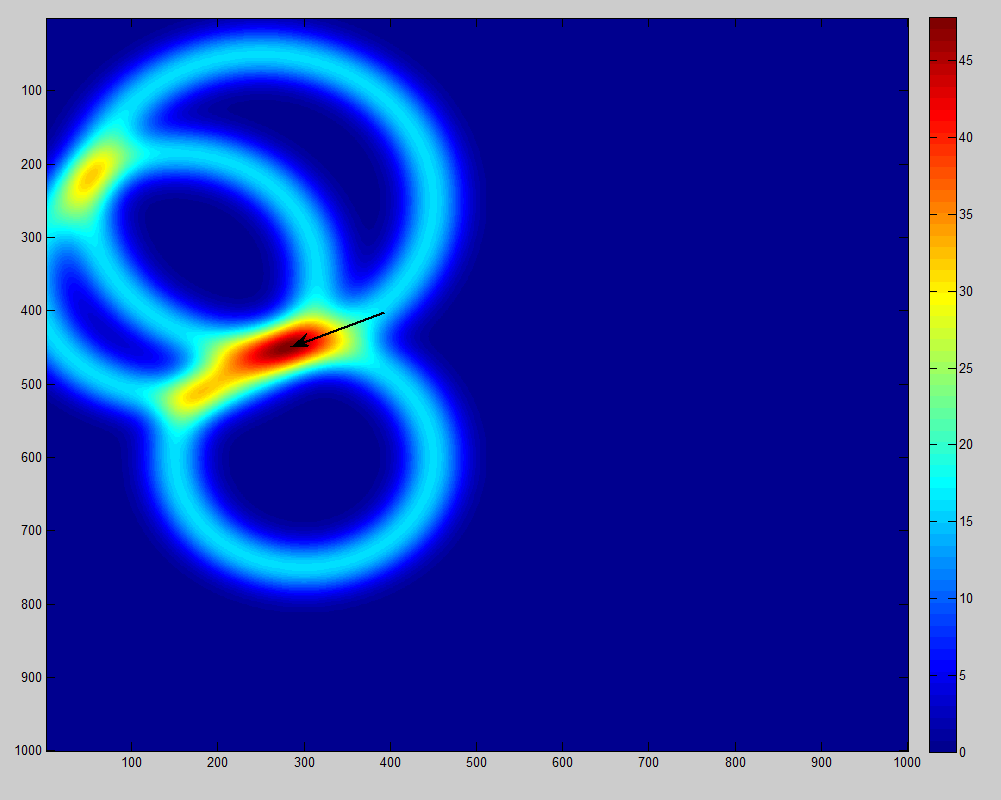
\includegraphics[width=0.75\textwidth]{guasianRouter}
\end{figure}
Zaprezentowany sposób wyznaczania lokalizacji dotyczył obliczeń w przestrzeni dwuwymiarowej. Przejście na przestrzeń trójwymiarową nie stanowi problemu - jedynymi zmianami, jakie należy wprowadzić, są:
\begin{itemize}
	\item wykonywanie obliczeń dla punktów $(X,Y,Z)$
	\item zmiana sposobu obliczania odległości euklidesowej między odbiornikiem, a transmiterem - należy wyznaczać odległość w przestrzeni trójwymiarowej.
\end{itemize}

\chapter{Propagacja sygnału radiowego}
\label{cha:teoria}
\section{Zanik sygnał radiowego}
Sygnał radiowy, wysłany przez urządzenie, w wyniku przechodzenia przez ośrodek (najczęściej jest nim powietrze) ulega zanikowi. Różnica w mocy sygnału odczytanego przez odbiornik, a siłą sygnału wysłanego przez nadawcę, pozwala na obliczenie odległości pomiędzy dwoma urządzeniami. Dodatkowymi współczynnikami, które mają wpływ na obliczenia, są:
\begin{itemize}
	\item zysk energetyczny anteny nadawcy oraz odbiorcy
	\item margines zaniku, który zależy od czułości odbiornika
	\item straty w sile sygnalu wynikające ze środowiska - przeszkody, odbicia, inne urządzenia nadające
\end{itemize}
\begin{figure}[H]			
	\centering
	\caption{Schemat zaniku sygnału}
	\includegraphics[width=0.75\textwidth]{zanik_sygnalu}
\end{figure}
\section{Zysk energetyczny anteny}
Zysk energetyczny anteny jest to stosunek mocy ateny wypromieniowanej w danym kierunku do mocy wypromieniowanej przez antenę wzorcową. Anteną wzorcową może być m.in. antena izotropowa, czyli antena bez fizycznych rozmiarów, która cały sygnał zasilany wysyła we wszystkich kierunkach. W takim wypadku, zysk energetyczny anteny wyrażany jest w $dBi$.\\
Na zysk energetyczny mają również wpływ kierunkowość oraz materiał, z którego wykonana jest antena.
\section{Margines zaniku}
Margines zaniku (fade margin) jest to wartość określająca wielkość "marginesu" pomiędzy wartością odebraną, a czułością odbiornika. Określa się ją wzorem:
\begin{equation}
FM = P_{rs} - P_{rx}
\end{equation}
gdzie $P_{rs}$ to siła odebranego sygnału.\\
Margines zaniku jest wyznacznikiem, jak "dobre" jest połączenie między transmiterem i odbiorcą. Czym wyższa wartość marginesu zaniku, tym bardziej niezawodne jest połączenie.
Wartość marginesu zaniku określa się w jednostce $dB$.
\section{Received signal strength indication}
Received signal strength indication (skrótem RSSI) jest to miara określająca moc sygnału odbieranego. Przyjmuje ona wartości niedodatnie (gdzie 0 oznacza sygnał najsilniejszy). Jednostką, w jakiej określa się siłę sygnału jest $dBm$, która jest logarytmiczną jednostką miary mocy odniesiona do mocy $1mW$.\\
System Android pozwala na odczytanie siły odbieranego sygnału. Można do tego wykorzystać API $WifiManager$ (w przypadku odczytu sygnału WiFi) oraz $BroadcastReceiver$ (w przypadku odczytu sygnału Bluetooth).
\section{Free-space path loss}		  		  
Utrata w sile sygnału spowodowana przejściem fali elektromagnetycznej przez ośrodek (najczęściej powietrze).
Wzór na obliczanie FSPL:
\begin{equation}
FSPL = P_{tx} + AG_{tx} + AG_{rx} - P_{rx} - FM - L
\end{equation}
%http://electronicdesign.com/communications/understanding-wireless-range-calculations
%Microwave and Millimetre-Wave Design for Wireless Communications  Autorzy Ian Robertson,Nutapong Somjit,Mitchai str 449
%https://en.wikipedia.org/wiki/Free-space_path_loss
%http://www.tplink.com/ie/support/calculator/#1
%http://stackoverflow.com/questions/11217674/how-to-calculate-distance-from-wifi-router-using-signal-strength
Gdzie symbole oznaczają:
\begin{itemize}
	\item $P_{tx}$ - siła trasmitera, wyrażona w dBm
	\item $AG_{tx}$ - zysk energentyczny anteny transmitera, wyrażony w dBi
	\item $AG_{rx}$ - zysk energentyczny anteny odbiorcy, wyrażony w dBi
	\item $P_{rx}$ - czułość odbiornika, wyrażona w dBm
	\item $FM$ - margines zaniku sygnału (fade margin) - określa jak duży jest margines różnicy pomiędzy uzyskaną siłą sygnału, a czułością odbiornika
	\item $L$ - straty wynikające np z oddziaływania innych transmiterów, przeszkód itp.
\end{itemize}
Dodatkowo, FSPL można obliczyć, używając następujący wzór:
\begin{equation}
FSPL = 20log_{10}\left(\frac{d}{d_{0}}\right) + 20log_{10}(f) + K
\end{equation}
%Indoor Localization Method Based on Wi-Fi Trilateration Technique Maxim Shchekotov
% Wi-Fi Indoor Positioning System Based on RSSI Measurements from Wi-Fi  Access Points  –  A Tri-lateration Approach Onkar Pathak, Pratik Palaskar, Rajesh Palkar, Mayur Tawari
Gdzie symbole oznaczają:
\begin{itemize}
	\item $d$ - dystans dzielący trasmiter od odbiorcy, wyrażony w metrach
	\item $d_{0}$ - dystans referencyjny -  w tym wypadku 1 metr
	\item $f$ - częstotliwość transmitera - wyrażona w MHz
	\item $K$ - stała, którą można określić wzorem:
	\begin{equation}
	K = 20log_{10}\left(\frac{4\pi d_{0}}{C}\right)
	\end{equation}
	gdzie $d_{0}$ to dystans referencyjny (taki sam jak we wzorze wyżej), a $C$ to długość fali emitowanej przez transmiter
\end{itemize}	  
Po przekształceniu wzoru, uzytkujemy:
\begin{equation}
d = 10^{\left(\frac{FSPL - K - 20log_{10}(f)}{20}\right)}
\end{equation}
A po połączeniu obu wzorów dostajemy:
\begin{equation}
d = 10^{\left(\frac{P_{tx} + AG_{tx} + AG_{rx} - P_{rx} - FM - L - K - 20log_{10}(f)}{20}\right)}
\end{equation}
Po podstawieniu wzoru na margines zaniku do wzoru (5), uzyskujemy
\begin{equation}
d = 10^{\left(\frac{P_{tx} + AG_{tx} + AG_{rx} - P_{rs} - L - K - 20log_{10}(f)}{20}\right)}
\end{equation}
\chapter{Testy sposobów komunikacji radiowej}
\label{cha:teoria}

Testy mają na celu zbadać skuteczność wyznaczania odległości między transmiterem, a odbiornikiem dla sygnałów Wifi i Bluetooth.\\
Testy odbywać się będą w dwóch etapach:
\begin{itemize}
	\item w pierwszym, odbiornik i transmiter będą oddalone od siebie o około 1m. Mierzona będzie siła odbieranego sygnału. Celem tego etapu jest określenie, jak duże straty siły sygnału związane są z komunikacją Wifi i Bluetooth. Straty mogą wynikać z izolacji obudowy, odbić, interferencji kilku fal lub z braku kierunkowości anteny (antena wbudowana).
	\item w drugim etapie, obliczone wcześniej wartości strat zostaną wykorzystane, aby zmierzyć, jak zmienia się siła sygnału, kiedy na drodze pojawi się przeszkoda. Do testów wykorzystana została książka o formacie A4 grubości 7 centymetrów, drewniane drzwi o grubości 5 centymetrów oraz ściana o grubości 26 centymetrów.
\end{itemize}
Uzyskane informacje pozwolą obliczyć współczynnik strat, jaki należy uwzględnić podczas późniejszego obliczania lokalizacji użytkowników oraz pozwoli przydzielić każdemu ze sposobów komunikacji radiowej odpowiednią wagę, w zależności od jego odporności na zakłócenia.
\section{Wykorzystane urządzenia}
\begin{enumerate}
	\item Smartphone Sony Xperia Z1 Compact (D5503) - odbiornik\\				
	Dane techniczne:
	\begin{itemize}
		\item Częstotliwość - 2,4GHz
		\item Przyrost siły sygnału z anteny WiFi - 2dBi
		\item Przyrost siły sygnału z anteny Bluetooth - 0dBi
	\end{itemize}
	\item Router TP-Link TD-W8970 - nadajnik\\
	Dane techniczne:
	\begin{itemize}
		\item Częstotliwość - 2,4GHz
		\item Dwie zewnętrzne anteny kierunkowe
		\item Przyrost siły sygnału z anteny - 4dBi
		\item Siła transmitera - 16.5dBm					
	\end{itemize}
	%\item Router TP-Link TL-WA701ND - nadajnik\\
	%Dane techniczne:
	%\begin{itemize}
	%	\item Częstotliwość - 2,4GHz
	%	\item Jedna zewnętrzna antena kierunkowa
	%	\item Przyrost siły sygnału z anteny - 2dBi
	%	\item Siła transmitera - 15dBm					
%	\end{itemize}
	\item Smartphone Samsung Grand 2 (G7102) - nadajnik\\
	Dane techniczne:
	\begin{itemize}
		\item Jedna antena wbudowana
		\item Przyrost siły sygnału z anteny - 0dBi
		\item Siła transmitera Bluetooth - 6dBm				
	\end{itemize}
\end{enumerate}
\section{Warunki}
Wszystkie pomiary wykonywane były w pomieszczeniu zamkniętym, bez przeszkód na drodze sygnału. Wszystkie urządzenia znajdowały się na tej samem wysokości, skierowane do siebie górną częścią obudowy (w przypadku routera, skierowany był on do odbiornika swoimi antenami kierunkowymi).
\begin{figure}[H]
	\centering			
	\caption{Zdjęcie urządzeń pomiarowych oraz środowiska testowego}
	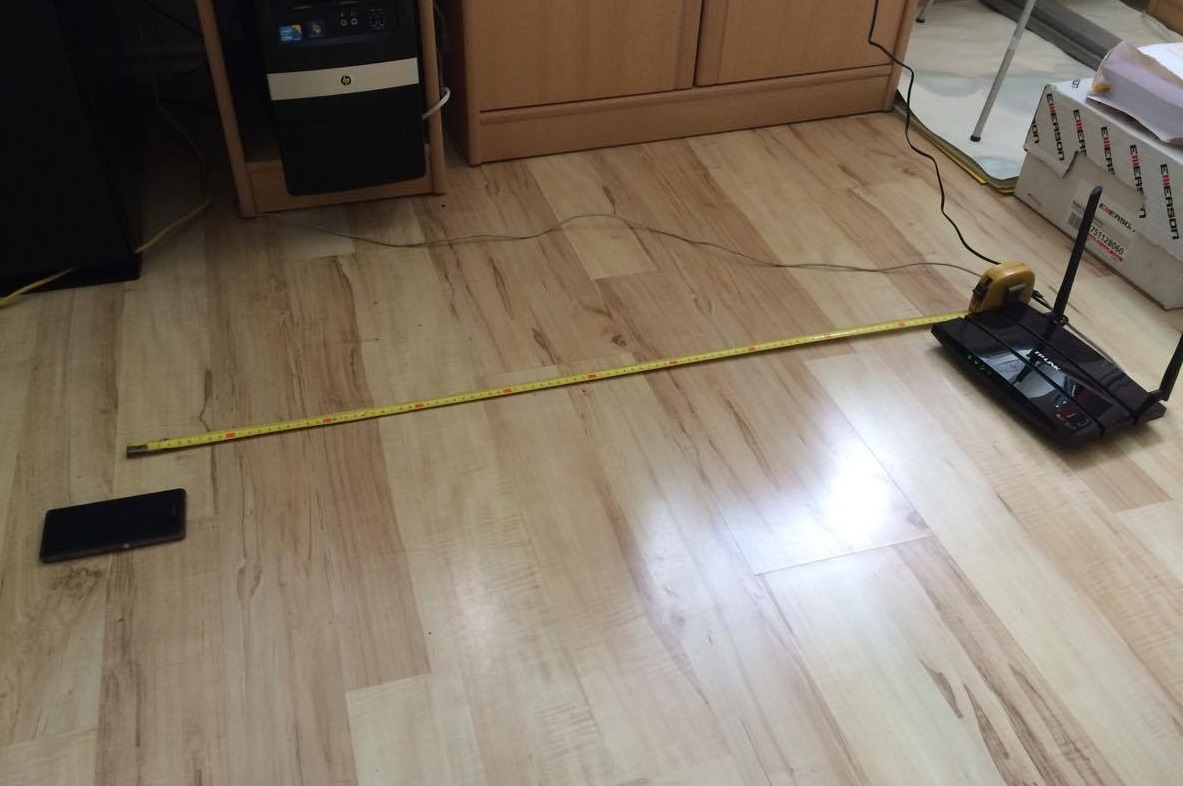
\includegraphics[width=0.75\textwidth]{srodowisko_pomiarowe}
\end{figure}
\section{Pobranie danych i analiza wyników}
Dla każdego eksperymentu została wykonana odpowiednio duża ilość powtórzeń (od 70 do 120), aby wynik był dokładniejszy. W tym celu, została stworzona lekka aplikacja, która pobierała zgłoszenia telefonu i zapisywała je do pliku tekstowego. Następnie, po skończonych testach, parsowała dane i wyliczała średnią dla sił sygnałów pochodzących z interesującego nas źródła (sygnały pochodzące z innych źródeł były odrzucane). Tak obliczone dane zostały zawarte w tabelach w dalszej części rozdziału.
\section{Wyznaczenie wartości strat}
Eksperyment polegał na ustawieniu transmitera w odległości 1 metra od odbiornika, na jednym poziomie, antenami do siebie. Na podstawie siły sygnałów obliczana została wartość strat, jakie musiałyby być uwzględnione, aby odległość obliczona równała się odległości fizycznej.\\			
\begin{figure}[H]
	\centering			
	\caption{Szkic eksperymentu nr 1}
	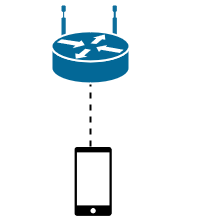
\includegraphics{exper1}
\end{figure}
\subsection{Pomiary}
	Wartości obliczone dla eksperymentu nr 1, w którym Router TP-Link TD-W8970 jest transmiterem sygnału Wifi, a Samsung Grand 2 transmiterem Bluetooth:
	\begin{center}
		\begin{minipage}{\linewidth}
			\begin{tabular}{|c|c|c|c|}
				\hline 
				Sygnał & Ilość prób & Średnia siła sygnału (w dBm) & Obliczona średnia wartość strat (dB) \\ 
				\hline 
				Wi-Fi & 163 & -38.88 & 21.18 \\ 
				\hline 
				Bluetooth & 113 & -57.5 & 23.3 \\ 
				\hline 
			\end{tabular} 
		\end{minipage} 
	\end{center}
\subsection{Wnioski}
Z danych uzyskanych podczas eksperymentu wynika, że straty spowodowane zakłóceniami sygnału Bluetooth są wyższe niż spowodowane zakłóceniami sygnału WiFi. Może się to wiązać z tym, że transmiter Wifi ma większą moc, zaś kierunkowe anteny zmniejszają ilość zakłóceń wynikających z odbicia się sygnału. Wartości strat obliczone dla obu sposobów komunikacji zostaną wykorzystane podczas eksperymentu nr 2 oraz będą miały wpływ na wybór wagi dla siły sygnałów podczas określania lokalizacji użytkowników.
\section{Przeszkody na drodze sygnału}
Drugi eksperyment ma na celu zbadanie odporności każdego z rodzajów sygnałów na zakłócenia związane ze stojącą na drodze przeszkodą. Wnioski z tego eksperymentu będą miały duży wpływ na działanie systemu, ponieważ w rzeczywistym środowisku, w którym ma działać tworzony system, transmiter od użytkownika będzie dzielić czasami nawet kilka ścian i ważne jest, aby odpowiednio dobrać wagi dla sygnałów.\\
W pierwszej części eksperymentu, transmiter został oddalony od odbiornika o 1 metr. Na drodze sygnału została postawiona gruba książka w formacie A4. W drugiej części eksperymentu, transmiter od odbiornika oddalony został o 2 metry, w taki sposób, aby na drodze sygnału znalazły się najpierw drewniane drzwi, a w kolejnej części eksperymentu ściana.\\
Do dokonania pomiarów zostały wykorzystane te same urządzenia jak w przypadku eksperymentu nr 1.\\
Wartość błędu bezwzględnego obliczana była na podstawie wzoru:
\begin{equation}
\delta = |D_r - D_o|
\end{equation}
gdzie $D_r$ to rzeczywista odległość między transmiterem, a odbiornikiem, zaś $D_o$ to odległość obliczona na podstawie siły sygnału.
\begin{figure}[H]
	\centering			
	\caption{Szkic eksperymentu nr 2}
	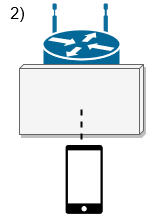
\includegraphics{exper2}
\end{figure}
\subsection{Pomiary}
Wartość siły sygnałów, obliczony dystans oraz wielkość błędu dla pomiaru sygnału Wifi i Bluetooth, dla którego przeszkodą była książka przy dystansie 1 metra:
\begin{center}
	\begin{minipage}{\linewidth}
		\begin{tabular}{|c|c|>{\centering} p{3cm}|>{\centering} p{3cm}|c|}
			\hline 
			Sygnał & Ilość pomiarów & Średnia siła sygnału (w dBm) & Średnia obliczona odległość (m) & Błąd bezwzględny (m)\\ 
			\hline 
			Wifi & 182 & -40,81 & 1,24 & 0,24 \\ 
			\hline 
			Bluetooth & 70 & -61.46 & 1,57 & 0,57 \\ 
			\hline 			
		\end{tabular} 
	\end{minipage} 
\end{center}
Wartość siły sygnałów, obliczony dystans oraz wielkość błędu dla pomiaru sygnału Wifi i Bluetooth, dla którego przeszkodą były drzwi przy dystansie 2 metrów:
\begin{center}
	\begin{minipage}{\linewidth}
		\begin{tabular}{|c|c|>{\centering} p{3cm}|>{\centering} p{3cm}|c|}
			\hline 
			Sygnał & Ilość pomiarów & Średnia siła sygnału (w dBm) & Średnia obliczona odległość (m) & Błąd bezwzględny (m)\\ 
			\hline 
			Wifi & 112 & -48,1 & 2,89 & 0,89 \\ 
			\hline 
			Bluetooth & 107 & -67,05 & 3,01 & 1,01 \\ 
			\hline 			
		\end{tabular} 
	\end{minipage} 
\end{center}
Wartość siły sygnałów, obliczony dystans oraz wielkość błędu dla pomiaru sygnału Wifi i Bluetooth, dla którego przeszkodą była ściana przy dystansie 2 metrów:
\begin{center}
	\begin{minipage}{\linewidth}
		\begin{tabular}{|c|c|>{\centering} p{3cm}|>{\centering} p{3cm}|c|}
			\hline 
			Sygnał & Ilość pomiarów & Średnia siła sygnału (w dBm) & Średnia obliczona odległość (m) & Błąd bezwzględny (m)\\ 
			\hline 
			Wifi & 103 & -48,3 & 2,96 & 0,96 \\ 
			\hline 
			Bluetooth & 110 & -66,95 & 2,97 & 0,97 \\ 
			\hline 			
		\end{tabular} 
	\end{minipage} 
\end{center}
\subsection{Wnioski}
Wyniki eksperymentu nr 2 jasno wskazują, że sygnał Wifi jest bardziej odporny na zmiany spowodowane pojawiającą się na drodze przeszkodą. Ma to duży wpływ na obliczanie lokalizacji użytkownika na podstawie sygnału i dlatego technologia Wifi będzie miała wyższą wagę w tworzonym systemie.\\
Dodatkowo, warto zwrócić uwagę, że błędy wynikające z obecności na drodze sygnału drzwi oraz ściany są mniejsze, niż można się było spodziewać. Może to wynikać z faktu, że sygnał nie rozchodzi się tylko w jednym kierunku i dzięki temu, podczas przechodzenia przez drzwi, część sygnału napotykała również na ścianę, co spowodowało większe zakłócenia.



% itd.
% \appendix
% \include{dodatekA}
% \include{dodatekB}
% itd.

\printbibliography

\end{document}
